In the latest years, several frameworks have gained popularity due to their ease of use and robust features, with Django being one of the most prominent~\cite{DJANGO-POP, DJANGO}. Django is a web framework built on Python, renowned for its simplicity, scalability, and rapid development capabilities. It provides a comprehensive set of tools and libraries that simplify the development process, including an \ac{orm} for database management, a powerful templating engine for user interface rendering, and a routing system for handling \acs{url} requests. Django follows the \ac{mvt} software design pattern, an extension of the traditional \ac{mvc} pattern.

\subsubsection{\acs{mvt} design pattern}

The \acl{mvt} pattern separates the different aspects of a web application, providing a structured approach for handling data (Model), presentation logic (View), and user interface (Template).

\begin{compactitem}[\textbullet]
    \item The \textbf{Model} interacts with the database. It defines the data structure and provides methods for querying, updating, and manipulating the database. When a \acs{url} is accessed, it is responsible for retrieving relevant data from the database or updating existing data depending on the request.
    \item The \textbf{View} handles the logic behind processing the user's request. After receiving the necessary parameters from the \acs{url} request, it interacts with the Model to retrieve or modify data as needed, and may perform additional operations based on the request parameters. Finally, the View prepares the data to be passed to the Template for rendering.
    \item The \textbf{Template} is responsible for handling the user interface. It defines the structure, layout, and presentation of the page, incorporating any necessary data from the View to populate the page with the requested information. Once the Template has processed the data, it generates the \acs{html} response to be sent back to the user's browser.
\end{compactitem}

\begin{figure}[Django's Model-View-Template architecture]{FIG:Django}{Django's \acl{mvt} architecture}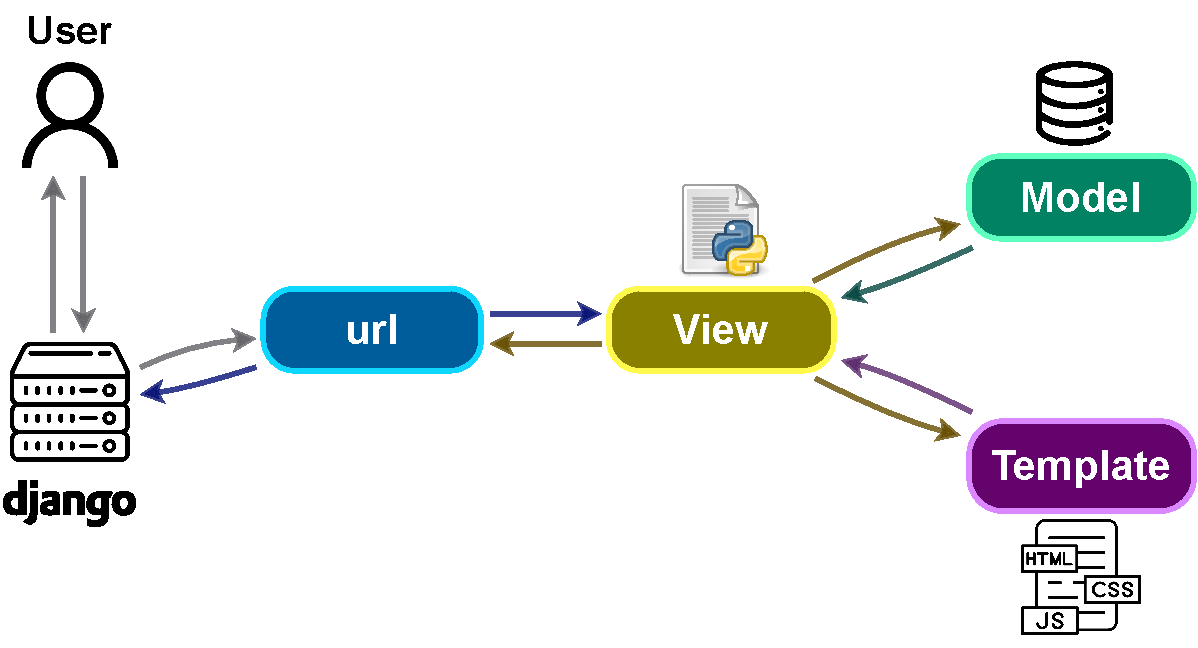
\includegraphics[width=0.7\textwidth]{img/Django.pdf}
\end{figure}

When users access a webpage built on Django, all pattern components work together to handle the requests and generate the corresponding responses, as depicted in Figure~\ref{FIG:Django}. This division of responsibilities allows for a clean separation of concerns and promotes code modularity and maintainability, making it easier to modify or update specific components without affecting the others.